\chapter{Prototypische Analyse}\label{analyse}

Das vorherige Kapitel hat gezeigt, welche Aspekte wie analysiert werden sollen. Diese Analyse wird jetzt entsprechend anhand von Codebeispielen oder Recherchen durchgeführt.

\section{Verbreitung und Ausgereiftheit}

Zuerst soll dabei betrachtet werden, wie weit die jeweiligen Technologien verbreitet sind. Da \ac{REST} als wesentlich ältere und nahezu konkurrenzlose Technologie im Raum stand, wird sich über das Warum hier kaum etwas sagen lassen. Interessanter sind dagegen Unternehmen, welche sich für einen Wechsel von \ac{REST} zu GraphQL entschieden haben. Ein nützlicher Aspekt ist es auch zu wissen, welche Bibliotheken existieren.

\subsection{Unternehmen}\label{unternehmen}

\textbf{Twitter:} Twitter ist das wohl bekannteste Beispiel einer REST-API. Sie erlaubt Entwicklern, nahezu alle Daten von Twitter auszulesen, ohne dabei auf der Twitter Website zu sein. Das Prinzip ist aber genau das gleiche: Eine Schnittstelle stellt bspw. das Login zur Verfügung. Der Token, der dabei als Antwort erzeugt wird, kann genutzt werden, um im eigenen Namen zu Tweets zu posten. Es können aber natürliche auch aktuelle Tweets der eigenen Twitter Timeline ausgelesen werden \parencite{Twitter2020}. Dabei werden die Designprinzipien von \ac{REST} von der Twitter-API nicht vollständig vollständig implementiert \parencite{Ullenboom2017}. Stattdessen nutzt die Implementierung nur die Aspekte, welche sie wirklich benötigt. \ac{REST} wird hier wahrscheinlich nur deswegen verwendet, weil es früher keine sinnvolle Alternative gab. \ac{SOAP}, welches von \ac{REST} vom Markt verdrängt wurde, hatte dem kaum was gegenüber zu setzen. Andere Unternehmen wie Github nutzen aber die neuen Alternativen, um die Technologie zu wechseln.\\
\\
\textbf{Github:} Github ist ein Unternehmen, welches eine Plattform zur Verfügung stellt, um die Entwicklung von Software zu organisieren. Beim Wechsel der \ac{api} von Version 3 auf Version 4 in 2016 wechselten sie auch von \ac{REST} zu GraphQL. Sie geben dafür mehrere Gründe an.\\
Der erste ist der sehr weitgefächerte Punkt der Skalierbarkeit. Skalierbarkeit hängt von vielen Faktoren ab, in ihrem konkreten Beispiel verweisen sie aber vor allem auf die Menge der gesendeten Daten und Anfragen. Das Kapitel \nameref{antwortzeit} hat schon beschrieben, dass es sich dabei um die Probleme des Over- und Underfetching handelt. Interessant ist aber, dass sie als Ursache für das Overfetching vor allem \ac{HATEOAS} kritisieren. Im Abschnitt \nameref{OverUnderfetching} werden diese Probleme genauer beleuchtet. Aus Githubs Perspektive löst GraphQL diese Probleme vollständig.\\
Das andere Problem, auf das Github genauer eingeht, ist komplizierter. Ihr Problem mit \ac{REST} ist, dass Informationen über Endpunkte nicht nur schwer zu erhalten, sondern auch schwer zu bestimmen sind. Als Beispiel nennen sie dafür die Bestimmung der Zugriffsrechte, welche für jeden Endpunkt nötig sind. Aber auch weitere Features, welche den Nutzen der \ac{api} vereinfachen, wie Typesicherheit von Userparametern oder automatische Dokumentation, hat ihnen bei \ac{REST} gefehlt. Das Kapitel \nameref{dokumentation} wird sich damit beschäftigen, wie diese Faktoren in GraphQL umgesetzt wurden und welche Vorteile sich daraus ergeben. \parencite{Github2020}
\\
\\
Weitere bekannte Unternehmen haben aus ähnlichen Gründen gewechselt. Dazu gehören Paypal, Airbnb und Shopify.

\subsection{Bibliotheken und Frameworks}

Viele Aspekte von \ac{REST} können durch Bibliotheken kaum unterstützt werden. Prinzipien wie \ac{HATEOAS} oder die Identifizierung der Ressourcen müssen beim Design der \ac{api} vom Entwickler selber bedacht werden.  Trotzdem versuchten verschiedene Frameworks Entwickler beim Aufbau einer REST-API zu unterstützen. Namentlich kann bspw. Spring Boot genannt werden. Dieses Framework ist für Java verfügbar. Spring Boot bietet viele Funktionalitäten an. Darunter gehört auch die Unterstützung für den Aufbau von REST-APIs. Neben der grundlegenden Implementierung vereinfacht Spring Boot bspw. auch die Validierung von User-Input \parencite{Spring2020}.\\
Insgesamt gesehen gibt es für jede anständige Programmiersprache eine REST-Imple\-mentierung mit mehr oder weniger Funktionalitäten. So hat Javascript das bereits erwähnte Express, während Python mit Flask aufwartet. \parencite{Slant2020}\\
GraphQL steht trotz der relativ kurzen Geschichte von fünf Jahren \ac{REST} kaum nach. Viele der etablierten Frameworks von \ac{REST} bieten inzwischen auch Lösungen für GraphQL an. So haben sowohl Spring Boot als auch Express Möglichkeiten, um eine GraphQL-API aufzubauen \parencite{Spring2020GraphQL} \parencite{GraphQL2020}. Insgesamt werden mehr als 20 Sprachen unterstützt \parencite{GraphQL2020Code}. Zusätzlich gibt es aber noch Bibliotheken, welche auf der Clientseite angewandt werden. Diese dienen einerseits dazu, die komplizierteren Anfragen übersichtlicher zu formulieren. Andererseits versuchen sie aber auch Probleme von GraphQL zu lösen. FlacheQL oder das bekanntere Appollo übernehmen bspw. das kompliziertere Caching von GraphQL(s. Kapitel \nameref{caching} für mehr Details) für den Nutzer \parencite{FlacheQL2019} \parencite{Apollo2020}. 

\subsection{Fazit}

Immer mehr Unternehmen wechseln bereits zu GraphQL. Und sie haben dafür gute Gründe. Dabei werden sie durch eine Vielzahl an Frameworks und Bibliotheken unterstützt. Bei nahezu jedem REST-Projekt kann theoretisch auf GraphQL gewechselt werden. Doch ob sich das für alle Unternehmen auch lohnt, werden die nächste Kapitel beleuchten.

\section{Implementierung}\label{Implementierung}

Wie in Kapitel \nameref{implementierung} angesprochen, wird sich diese Analyse nur mit einer einfachen Implementierung beschäftigen. Dafür soll sowohl hier als auch in den weiteren Abschnitten die Routen-API genutzt werden. 

\subsection{Routen-API}

Die Routen-API ist eine \ac{api} zur Verwaltung von Routen. Sie kann in der SignalK-API als Plugin hinzugefügt werden. Der Nutzer kann in der REST-Implementierung auf verschiedene Endpunkte zugreifen. Die Tabelle \ref{tab:Endpunkte} zeigt, welche Möglichkeiten dafür zur Verfügung stehen.

\begin{table}[h]
\begin{tabular}{p{3cm} p{3cm} p{7cm}}
Endpunkt & Methode & Funktionalität \\
\verb+/route+ & POST & Fügt eine neue Route hinzu \\
\verb+/route/{uuid}+ & PATCH & Aktualisiert eine vorhandene Route \\
 & GET & Gibt die Daten einer Route aus \\
 & DELETE & Löscht eine Route \\
\verb+/routes+ & GET & Gibt alle abgespeicherten Routen zurück
\end{tabular}
\caption{Routen-API: Endpunkte}
\label{tab:Endpunkte}
\end{table}

Wie die Datenstruktur einer solchen Route aufgebaut ist, kann im Code \ref{lst:RouteDaten} gesehen werden.

\begin{lstlisting}[caption={Beispiel Datenstruktur für eine Route},captionpos=b,label=lst:RouteDaten] 
	route {
		uuid: 'aeedd10s11223as',
		geometry: {
			coordinates: [[221.365, 200.233] [101.244, 135.313]]
			distance: 1048.231,
		},
		start: 'Kiel',
		end: 'Stockholm',
		description: 'Ostsee',
		name: 'Ostsee Toern',
		timestamp: '1593076241483.0'
	}
\end{lstlisting}

\subsection{Implementierung}

Für die Implementierungsanalyse soll nun der \textit{/routes}-Endpunkt genauer betrachtet werden. Ohne \ac{HATEOAS} würde die Datenstruktur der Antwort ungefähr wie der Code \ref{lst:RouteListDaten} aussehen. Weitere Felder wurden aus Platzgründen weggelassen. Der Code \ref{lst:RESTServer} zeigt dabei, wie dieser Fall in einer REST-API umgesetzt werden kann. Mit Express besteht ein solcher Endpunkt nur aus zwei Teilen. Zum Einen muss der \ac{URL} des Endpunktes angeben werden, welcher angibt, wohin der Client seine Anfrage schicken muss, um diesen Endpunkt anzusprechen. Außerdem noch die Funktion angegeben werden, welche aufgerufen wird, sobald eine Anfrage am Endpunkt ankommt. Mögliche Parameter der Anfrage werden durch die Übergabeparameter der Funktion übergeben. Da die endgültige Datenabfrage an die Datenbank für \ac{REST} und GraphQL identisch ist, kann die genaue Syntax ignoriert werden. Deswegen wird sie durch den Aufruf \textit{db.getRoutesData()} abgehandelt.

\begin{lstlisting}[caption={Beispiel Datenstruktur für eine Liste von Routen},captionpos=b,label=lst:RouteListDaten] 
	routes: [
		route {
			name: 'Ostsee',
			start: 'Kiel',
			end: 'Stockholm',
			...
		},
		route {
			name: 'Nordsee',
			start: 'Dangast',
			end: 'Langeoog',
			...
		}
	]
\end{lstlisting}

\begin{lstlisting}[caption={REST Server Implementierung},captionpos=b,label=lst:RESTServer] 
	app.get('/routes', async function (req, res, next) {
		var result = await db.getRoutesData()
		return res.json(result)
	})
\end{lstlisting}

Diese sehr einfache Variante funktioniert nur in Sprachen, wo der Rückgabetyp nicht explizit angeben werden muss. Andere Programmiersprachen wie Java schreiben vor, dass die genaue Datenstruktur der Antwort vorher definiert werden muss. Das ist aber eigentlich kein zusätzlicher Aufwand. Denn wie bereits in Kapitel \nameref{Dokumentation} erklärt wurde, muss diese Datenstruktur in der Dokumentation sowieso aufgeführt werden.  Nur dann können Anwender die \ac{api} wirklich effizient nutzen.\\
Bei GraphQL ist die Datenstruktur immer Teil der Implementierung. Dafür muss ein Schema definiert werden. Doch das Schema gibt nicht nur die Datenstruktur vor, es zeigt auch an, wie Anwender auf die \ac{api} zugreifen können. Dafür gibt es theoretisch zwei Möglichkeiten: 

\begin{itemize}
\item \textit{Query:} Eine Query entspricht dem Äquivalent einer \textit{HTTP-GET}-Abfrage, d.\,h. dass hier nur Daten zurückgegeben werden. Falls also niemand anders die Daten der Datenbank verändert, müssen die gleichen Queries auch die gleichen Daten zurückliefern. Will man die Daten verändern, benötigt man eine Mutation.
\item \textit{Mutation:} Eine Mutation erfüllt die Aufgabe mehrere   HTTP-Methoden. Denn eine Mutation ist jede Anfrage, welche die Daten im Backend verändert. Das können Updates verschiedener Parameter sein, aber auch das Löschen eines Objekts.
\end{itemize}
Um in GraphQL die gleiche Funktionalität wie der REST-Server zur Verfügung zu stellen, muss ein entsprechender Server aufgesetzt werden. Der Code \ref{lst:GraphQLServer} zeigt, wie das Ergebniss aussehen könnte. Der Endpunkt hat dabei mehrere Teile, und zwar einerseits wieder die \ac{URL}, welche jedoch auf den immer gleich bleibenden GraphQL-Endpunkt verweist. Außerdem wird der Endpunkt mit dem Schema und einem Resolver verknüpft. Der Resolver parst die Anfrage, gibt sie an die entsprechenden Funktionen weiter und baut am Ende die richtige, benötigte Datenstruktur für die Antwort zusammen. Als letzter Punkt wird noch \textit{graphiql} erwähnt. Dieses übersichtliche \ac{UI} hilft bei der korrekten Formulierung der Anfragen. Genauer wird sie im Kapitel \nameref{dokumentation} behandelt.

\begin{lstlisting}[caption={GraphQL Server Implementierung},captionpos=b,label=lst:GraphQLServer] 
	var schema = buildSchema(`
		type Query {
			routes: [Route],
		},

		type Route {
			uuid: String,
			geometry: GeometryObject,
			start: String,
			end: String,
			description: String,
			name: String,
			timestamp: String
		},

		type GeometryObject {
			coordinates: [[Float]],
			distance: Float
		}
	`);

	var resolver = {
		async routes(args) {
			var result = await db.getRoutesData()
		}
	}

	app.use('/graphql', graphqlHTTP({
		schema: schema,
		rootValue: resolver,
		graphiql: true,
	}));
\end{lstlisting}

Auf den ersten Blick ist diese Implementierung des GraphQL-Servers wesentlich aufwändiger. Wenn man jedoch bedenkt, dass die Datenstruktur des Schemas so oder zumindest so ähnlich auch für die Dokumentation der ersten Variante geschrieben werden muss, ist der Aufwand kaum größer.  Die \ac{SDL}, welche genutzt wird, um die Schemata aufzubauen, erlaubt aber noch kompliziertere Strukturen. So können bspw. Interfaces genutzt werden, um den grundlegenden Aufbau mehrerer Typen festzulegen. Die meisten Strukturen dürften einem Entwickler bekannt vorkommen. Da sie aber mit \ac{SDL} in einer neuen Programmiersprache formuliert werden müssen, muss diese am Anfang auch erst gelernt werden. \\
Wenn man vom Schema absieht, ist der größte Unterschied, dass bei der ersten Variante der spezifische Endpunkt \textit{/routes} angefragt wird, wie es im Code \ref{lst:RESTClient} zu sehen ist. Bei weiteren Funktionalitäten, welche sich mit Routen beschäftigen, müsste ein anderer Endpunkt angefragt werden. Bei GraphQL hingegen wird immer der \textit{graphql} Endpunkt angefragt. Im Nachrichtenrumpf der Anfrage wird dann genauer spezifiziert wird, was gesucht wird. Ein Beispiel hierfür zeigt der Code \ref{lst:GraphQLClient}. 

\begin{lstlisting}[caption={REST Client Implementierung},captionpos=b,label=lst:RESTClient] 
	fetch('http://localhost:3000/routes')
		.then(r => r.json())
		.then(data => {
			console.log(data);
		});
\end{lstlisting}

\begin{lstlisting}[caption={GraphQL Client Implementierung},captionpos=b,label=lst:GraphQLClient] 
	fetch('http://localhost:3000/graphql', {
	   	method: 'POST',
	    	headers: {
	      		'Content-Type': 'application/json',
	    	},
	    	body: JSON.stringify({
	      		query: `
	      			query { 
					routes { 
						uuid, 
						name,
						...
					} 
				}
			`
		})
	})
		.then(r => r.json())
		.then(data => {
			console.log(data)
		});
\end{lstlisting}

Bei den Clientanfragen sind die Unterschiede schon wesentlich deutlicher. Der REST-Endpunkt gibt unabhängig von der Anfrage immer die gleichen Daten zurück. Entsprechend können die Anfragen auch sehr klein gehalten werden. Die einzigen beiden Änderungen, welche realistisch wären, wären einerseits eine Angabe, welches Dateiformat als Antwort erwartet wird. Das könnte z. B. JSON oder XML sein. Andererseits könnten noch mögliche HTTP-Header gesetzt werden, um Caching zu ermöglichen. Das Kapitel \nameref{caching} beschäftigt sich genauer damit. Bei GraphQL muss genau angeben werden, was benötigt wird. Dafür wird die namensgebende \textit{Graph Query Language} verwendet. Um den Code kleiner zu halten, wurde hierbei auf eine vollständige Aufzählung aller Felder verzichtet. Falls man aber wirklich die gleichen Daten benötigt, welche auch die REST-Schnittstelle ausgibt, müsste man alle Felder angeben. Die resultierenden Anfragen sind dadurch aber auch wesentlich größer. Für einen unerfahrenen Entwickler kommt hier das gleiche Problem auf, welches schon beim Server aufgetreten ist. Auch hier muss für eine effiziente Nutzung von GraphQL erst eine eigene Sprache gelernt werden. In vielen Faktoren ist diese zwar selbsterklärend, an \ac{REST} kommt sie damit aber nicht heran.\\
Zusammengefasst lässt sich sagen, dass als Entwickler ohne Erfahrung der Einstieg in \ac{REST} wesentlich einfacher ist. Ein Blick in die Dokumentation und es können Abfragen abgeschickt werden. Bei GraphQL ist der Einstieg ein wenig höher. Da aber weder \ac{SDL} noch die \text{Graph Query Language} wirklich kompliziert ist, hält sich der Aufwand auch hier in Grenzen. Doch auch bei erfahrenen Entwicklern sind die GraphQL-Anfragen immer noch aufwändiger als die REST-Anfragen.

\section{Dokumentation}\label{dokumentation}

Das vorherige Kapitel hat die Notwendigkeit einer Dokumentation schon angeschnitten. \ac{HATEOAS} und das GraphQL-Introspektionssystem sollen hier unterstützend sein. Doch wie funktionieren sie eigentlich genau und wie hilft das bei der Dokumentation?:\\

\textbf{HATEOAS:} \ac{HATEOAS} gibt an, dass die Antworten von REST-Servern Links enthalten sollen. Diese Links sollen entweder auf verwandte Ressourcen oder auf mögliche andere Funktionalitäten verweisen. Dabei sollen alle Möglichkeiten abgedeckt werden, welche der Anwender im Frontend zum aktuellen Zeitpunkt realistischerweise auswählen könnte. Dieses Verfahren hat theoretisch zwei Vorteile. Man könnte bspw. ein Frontend aufbauen, welcher nur die Links verwendet, um dem Nutzer zu zeigen, was er tun kann. Eine wirkliche \ac{UI} ist damit aber nicht möglich. Denn man weiß ja im vornerein gar nicht, welche Daten ankommen. Entsprechend kann man sie auch nicht übersichtlich darstellen.\\
Die andere Möglichkeit ist es, dass ein Entwickler einen Einstiegspunkt wählt und von diesem aus Schritt für Schritt alle Funktionalitäten der \ac{api} kennenlernt. Doch wer würde lieber mehrere Anfragen verschicken, als einmal in eine übersichtliche Dokumentation zu schauen, um eine Übersicht über die eigenen Möglichkeiten zu bekommen?\\
Zusammengefasst lässt sich sagen, dass \ac{HATEOAS} als Dokumentationsersatz unbrauchbar ist.\\
\\
\textbf{Introspektionssystem:} Das Introspektionssystem eröffnet die Möglichkeit, das komplette Schema  der vorliegenden GraphQL-API auszulesen. Da im Schema auch die Zugriffspunkte für die \ac{api} definiert werden, deckt diesem System eigentlich alle grundlegenden Funktionen ab, welche für eine Dokumentation benötigt werden. Sendet man aber eine Anfrage, welche wirklich alle Daten erhält, ab, ist die Antwort ziemlich unüber\-sichtlich. GraphiQL ist eine \ac{UI}, welche Abhilfe verschaffen soll. Sie ist in allen Implementierungen standartmäßig dabei und muss nur aktiviert werden. Das \ac{UI} gibt einem dabei die Möglichkeit, im Browser Anfragen zu formulieren und abzuschicken. Gleichzeitig stellt es eine interaktive Form des Schemas zur Verfügung. Auch Kommentare im Schema werden hier mit ausgegeben. Nutzt man also ein gut auskommentiertes Schema, wird die Dokumentation komplett automatisiert. Ein Schemausschnitt wie der Code \ref{lst:Kommentare} würde eine GraphiQL Dokumentation, wie in Abbildung \ref{fig:graphiql} zu sehen ist, erzeugen: 

\begin{lstlisting}[caption={Schema mit Kommentaren},captionpos=b,label=lst:Kommentare] 
"""Eine Route"""
	type Route {
		"""Identifikator"""
		uuid: String,

		"""Koordinatendaten"""
		geometry: GeometryObject,

		"""Startort"""
		start: String,	
		...
\end{lstlisting}
\begin{figure}
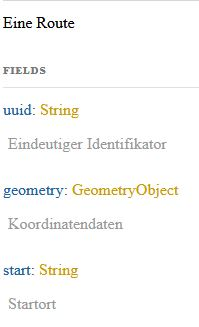
\includegraphics{graphiql}
\caption{GraphiQL Dokumentation}
\label{fig:graphiql}
\end{figure}

Beim grundlegenden Design ist GraphQL also wesentlich hilfreicher, was den Aufbau einer übersichtlichen Dokumentation angeht. Bibliotheken können aber beiden Technologien weiterhelfen. Bei GraphQL dienen Bibliotheken wie \textit{graphql-docs}  hauptsächlich dazu, die GraphiQL-\ac{UI} in eine übersichtliche Dokumentarform zu bringen \parencite{graphqlDocs2016}. Diese kann dann auch unabhängig vom Server genutzt werden. Bei \ac{REST} bieten Tools wie \textit{Swagger} eine automatisierte Dokumentation der eigenen \ac{api} an \parencite{Swagger2020}. Damit wird eigentlich die gesamte Dokumentationsfunktionalität von GraphiQL abgedeckt.\\
Zusammengefasst lässt sich sagen, dass das Introspektionssystem und die darauf aufgebaute GraphiQL-\ac{UI} bereits eine ausführliche automatisierte Dokumentation ermöglicht. Um mit \ac{REST} auf das gleiche Niveau zu kommen, müssen externe Bibliotheken genutzt werden. Diese bieten dann aber auch äquivalente Funktionalitäten oder sogar mehr an.

\section{Validierung}\label{validierung}

Das Typesystem wird von GraphQL nicht nur für die Introspektion verwendet. GraphQL nutzt es auch, um Anfragen automatisch zu validieren. Damit kann die Struktur der Query, welche durch die \textit{Graph Query Language} festgelegt wird, validiert werden. Ein Entwickler muss bei Anfragen also nicht überprüfen, ob sie vom Schema erfüllt werden können.\\
Zusätzlich garantiert GraphQL mit dem Typesystem auch, dass alle eingegebenen Parameter und Daten den richtigen Datentyp haben. Bei \ac{REST} muss diese Überprüfung, manuell durchgeführt werden. Meistens ist das jedoch der einfache Teil der Validierung. Denn in vielen Fällen unterliegen die Daten noch Einschränkungen, welche sie erfüllen müssen. Ein E-Mail String sollte bspw. nicht jeder beliebige String sein, sondern nur ein String, welcher folgenden Regexausdruck erfüllt: 

\begin{quote}
\verb; \b[A-Z0-9._%+-]+@[A-Z0-9.-]+\.[A-Z]{2,}\b;
\end{quote}

Diese Validierung lässt sich sowohl bei \ac{REST} als auch bei GraphQL ohne Bibliotheken nur sehr aufwändig umsetzten. Denn alle Parameter müssen mühsam mit \textit{if-Anweisun\-gen} validiert werden. Das ist nicht nur unübersichtlich, sondern es führt auch sehr wahrscheinlich zu sich wiederholenden Code. Auf die Art und Weise würden somit nur sehr einfache und wenige Validierung umgesetzt. Meisten werden deswegen Bibliotheken genutzt, welche sich in vielen Faktoren ähnlich sind. Spring Boot bietet bspw. eine Validierungslösung für beide Technologien an. Werden also Validierung benötigt, die über eine Datentyp-Validierung hinausgehen, hat keine der Technologien einen entscheidenden Vorteil.

\section{Antwortzeit}

Auch eine ausführliche Dokumentation und einfache Implementierung helfen nicht, wenn die die Antwortzeit zu hoch und der Client entsprechend unzufrieden ist.

\subsection{Over- und Underfetching}\label{OverUnderfetching}

Die komplizierteren Anfragen der GraphQL-Implementierung können benutzt werden, um sowohl Over- als auch Underfetching zu umgehen. Bei \ac{REST} muss hingegen die Implementierung so designt werden, dass diese Probleme möglichst klein gehalten werden. 

\subsubsection{Overfetching} Für einen Overfetching-Fall könnte man einfach eine Erweiterung der Funktionalität des Kapitels \nameref{Implementierung} betrachten. Zusätzlich zu allen Daten der Routen will jetzt ein Frontend diese Routen auflisten. Dafür werden aber nur der Name und der Start- und Endpunkt benötigt. Für GraphQL würde sich dabei nichts ändern. Eine Anfrage wie im Code \ref{lst:GraphQLOverfetching} zu sehen ist, würde diese Anforderungen exakt erfüllen.

\begin{minipage}{\linewidth}
\begin{lstlisting}[caption={Client Anfrage welche nur drei Felder pro Route zurückgibt},captionpos=b,label=lst:GraphQLOverfetching] 
	query { 
		routes { 
			name, 
			start,
			end
		}
	} 
\end{lstlisting}
\end{minipage}

Bei \ac{REST} ist die Lösung nicht so einfach. Würde man hier keine Änderungen durchführen, hätte man nur die Anfrage des Codes \ref{lst:RESTClient} zur Verfügung. Diese würde aber natürlich viel zu viele Daten für jede Route ausgeben. Es gibt für \ac{REST} aber einige Lösungsansätze, um das Problem zu umgehen:\\
\\
\textbf{Zusätzliche Endpunkte:} Diese Variante ist wohl die am weitesten verbreitete und auf den ersten Blick logischste. Jeder neue Fall wird einfach mit einem weiteren Endpunkt abgedeckt, welcher nur die benötigten Daten liefert. Dabei würde sich in vielen Fällen nur der Datenbankzugriff ändern. Der Code \ref{lst:RESTOverfetching1} zeigt dabei, dass die Implementierung nahezu identisch zum \ref{lst:RESTServer} Code aussehen würde. Eine Anfrage würde entsprechend nur an diesen neuen Endpunkt weitergleitet.\\

\begin{lstlisting}[caption={REST Server Implementierung},captionpos=b,label=lst:RESTOverfetching1] 
	app.get('/routesList', async function (req, res, next) {
		var result = await db.getRoutesListData()
		return res.json(result)
	})
\end{lstlisting}

Allerdings hat diese Variante zwei entscheidende Nachteile. Zum einen würde die Anzahl der Endpunkte im Laufe der Entwicklung drastisch zunehmen. Dadurch würde einerseits der Entwicklungsaufwand des Servers steigen, andererseits würde die Nutzbarkeit der \ac{api} eingeschränkt werden. Denn ein Frontendentwickler müsste sich jetzt durch eine immer komplizierter werdende Dokumentation durchschlagen, um den einen perfekt passenden Endpunkt auszuwählen. Das andere Problem liegt vor, wenn man die \ac{api} auch öffentlich zur Verfügung stellt. Hier kann man gar nicht für jeden Fall einen Endpunkt zur Verfügung stellen, da man gar nicht weiß, was alles benötigt wird. Dadurch wäre die Entwicklung eines Projektes mit diesem Verfahren sehr aufwändig und eingeschränkt.\\
\\
\textbf{Feldparamter:} Eine weitere Möglichkeit wäre die Nutzung eines zusätzlichen Parameters. Dieser würde dabei die Funktionalität von GraphQL imitieren. Der Client könnte diesen Parameter nutzen, um anzugeben, welche Felder er erhalten will. Der Code \ref{lst:FieldParamterClient} zeigt wie eine Anfrage aussehen könnte, welche an einen Server wie \ref{lst:FieldParamterServer} gesendet werden würde, um unseren Anwendungsfall abzudecken.\\
\begin{lstlisting}[caption={Client Anfrage mit Feldparametern},captionpos=b,label=lst:FieldParamterClient] 
	fetch('http://localhost:3000/routes/name,start,end')
\end{lstlisting}
\begin{lstlisting}[caption={Server Implementierung für Feldparameter},captionpos=b,label=lst:FieldParamterServer] 
	app.get('/routes/:fields', async function (req, res, next) {
                var results = await db.getRoutesData()
                var answers = [];
                var fields = req.params.fields;
                if (fields) {
                    fields = req.params.fields.split(',')
                    for (const result of results) {
                        var answer = {};
                        const keys = Object.keys(result)
                        for (const key of keys) {
                            if (fields.includes(key)) {
                                answer[key] = result[key];
                            }
                        }
                        answers.push(answer);
                    }
                }
                return res.json(answers)
            })
\end{lstlisting}

Doch auch hier zeigen sich schnell die Nachteile dieser Variante. Zum einen ist diese Implementierung wesentlich aufwändiger und unübersichtlicher. Für jeden Endpunkt, welcher diese Funktionalität zur Verfügung stellt, müsste entsprechend auch die Implementierung angepasst werden. Dabei deckt diese Variante nicht mal den gleichen Bereich ab, wie es GraphQL tun würde. Denn es können hier nur Felder ausgewählt werden, welche den primären Feldern der Datenstruktur entsprechen. Will man jetzt bei den Routendaten vom Code \ref{lst:RouteDaten} nur die Koordinaten der Route haben, müsste das ganze Feld \textit{Geometry} auswählt werden und somit auch alle weiteren Daten, die darin enthalten sind. Zusätzlich ist diese Variante auch wesentlich anfälliger für Fehler. Der Entwickler muss dabei genau mit der Dokumentation arbeiten, um die exakten Feldernamen zu nutzen und das Backend sollte wahrscheinlich eine Form der Validierung für diese Parameter aufbauen.\\
\\
\textbf{HATEOAS:} Als Ursache mancher dieser Probleme können die REST-Prinzipien hergenommen werden. Der Abschnitt \nameref{unternehmen} zeigt bereits, dass Github vor allem \ac{HATEOAS} als Ursache sieht. Für eine vollständige RESTful-API wäre die Liste, welche \textit{/routes} ausgibt, keine Liste aus vollständigen Routenobjekten. Stattdessen wären nur ein Link und einige wenige identifizierende Daten für jede Route vorhanden. Zusätzlich wären noch weitere Links auf verwandte Ressourcen oder Funktionalitäten Teil der Antwort, wie z.\,B. das Hinzufügen einer neuen Route mit \textit{/route}. Dadurch würde eine mögliche Antwort wie der Code \ref{lst:HATEOASDaten} aussehen. Das Problem des Underfetching, welches dabei auftritt, wird in Sektion \nameref{underfetching} behandelt. Das entscheidende Problem beim Overfetching sind die verwandten Ressourcen und Funktionalitäten. Bei einer stark vernetzten \ac{api} kann es schnell vorkommen, dass hierbei eine unglaubliche Menge an Daten in Form von Links mitgeschickt wird. Doch damit sich das wirklich lohnt, müsste das Frontend diese Links auch aktiv nutzen. Doch wie schon das Kapitel \nameref{dokumentation} gezeigt hat, hat dies kaum einen Mehrwert. Viele Entwickler nutzten die Dokumentation, um die Links direkt in den Code zu schreiben. Trotzdem müssen sie sich noch mit der ganzen Liste an Links rumschlagen, die mitgeschickt wird. Würde man \ac{HATEOAS} hier entfernen, wäre eine ausführliche Dokumentation vonnöten. Da dies aber eigentlich Grundvoraussetzung für jede \ac{api} ist, wäre das kein Hindernis. Gleichzeitig ist \ac{HATEOAS} nach \parencite{Fielding2008} eines der Kernprinzipien von \ac{REST} und somit wäre eine \ac{api} ohne \ac{HATEOAS} eigentlich auch keine REST-API mehr. Falls \ac{HATEOAS} also wirklich ein Hindernis darstellt, sollte man vielleicht Github folgen und auf GraphQL wechseln.

\vspace{-1pt}%

\begin{lstlisting}[caption={Beispielliste der Routen mit HATEOAS},captionpos=b,label=lst:HATEOASDaten]
	routes : {
		self: {
			href:			  '/routes'
			addRoute:		'/routes'
		}
		data: [
			{
				uuid:		  '3f441c99-67c1-48cd-8e97-9db483621eff'
				name:		  'Ostsee'
				get:		  '/routes/3f441c99-67c1-48cd-8e97-9db483621eff'
				delete:	  '/routes/3f441c99-67c1-48cd-8e97-9db483621eff'
				patch:		'/routes/3f441c99-67c1-48cd-8e97-9db483621eff'
			},
			{
				uuid:		  'abcde-67c1-48cd-8e97-9db483621eff'
				name:		  'Nordsee'
				get: 		  '/routes/abcde-67c1-48cd-8e97-9db483621eff'
				delete: 	'/routes/abcde-67c1-48cd-8e97-9db483621eff'
				patch: 	  '/routes/abcde-67c1-48cd-8e97-9db483621eff'
			}
		]
	}
\end{lstlisting}


Alle Varianten haben somit ihre Nachteile und sind kein äquivalenter Ersatz zu GraphQL. Eine beliebte Lösung ist eine Mischung aus verschiedenen Varianten. So können bspw. einige sicher benötigte Fälle mit individuellen Endpunkten abgehandelt werden. Zusätzlich werden noch weitere Endpunkte zur Verfügung gestellt, welche größere Mengen an Daten zurückgeben. Hierbei wird, wenn es möglich, nützlich und nicht zu aufwändig ist, mit Feldparametern gearbeitet.

\subsubsection{Underfetching}\label{underfetching}

Underfetching baut theoretisch auf den gleichen Problemen auf wie das Overfetching. Wie bereits erwähnt, könnte ein Underfetching-Fall bspw. auftreten, wenn die Liste des \textit{/routes}-Endpunktes das \ac{HATEOAS}-Prinzip erfüllt. Der Code \ref{lst:HATEOASDaten} macht dabei nochmal deutlich, dass die Daten, welche für jede Route geschickt werden, nur sehr begrenzt sind. Wenn der Anwender jetzt alle Daten für alle Routen haben will, muss er erst eine Anfrage an den  \textit{/routes}-Endpunkt abschicken, um alle Routen zu erhalten. Anschließend muss für jede Route eine individuelle Anfrage an den \verb+route/{id}+ geschickt werden, um die Daten der Routen zu erhalten. Dieses Problem ist als N+1-Problematik bekannt, d.\,h. um die Daten von N Routen zu erhalten, muss ich N+1 Anfragen abschicken \parencite{Kheyrollahi2014}.

Wendet man \ac{HATEOAS} vollständig an, lässt sich das Problem kaum umgehen. Die einzige Lösung wäre es, die Menge an Daten, welche in der Routenliste zurückgegeben werden, zu erhöhen. Damit könnten wieder häufige Anwendungsfälle abgedeckt werden. Wenn also bei der Diskussion mit den Anwendern herauskommt, dass sie eigentlich immer den Start- und Endpunkt der Route benötigen, können diese einfach direkt beim \textit{/routes}-Aufruf zurückgegeben werden. Dabei treten jedoch wieder zwei Probleme auf. Einerseits führen mehr Daten unweigerlich auch zu mehr Overfetching. Das sollte jedoch nach Möglichkeit vermieden werden. Und andererseits haben wir wieder das Problem, dass diese Informationen häufig gar nicht vollständig vorliegen. Entwickler, welche nicht an der \ac{api} beteiligt sind, sie aber für ihr Frontend nutzen, könnten ihre Datenwünsche nur beschränkt mitteilen. Und wenn man dann noch versucht, alle Wünsche zu erfüllen, könnte man einerseits auf \ac{HATEOAS} ganz verzichten und andererseits hätte man wieder ein Overfetchingproblem.\\
\\
Bei GraphQL ist Underfetching kein Problem. Das hat zwei Ursachen:
\begin{itemize}
\item \textbf{Datenstruktur als Graph:} Zu einem gewissen Grad versucht GraphQL das gleiche zu erreichen wie \ac{HATEOAS}. Doch statt mit Links sind Datenstrukturen, welche nahe beiander liegen, direkt verwandt. Mittels einer Query können dann alle diese verwandten Daten ausgelesen werden. Der Code \ref{lst:GraphQLServer} zeigt, wie eine einfache Implementierung dafür aussehen könnte.
\item \textbf{Mehrere Queries:} Doch auch wenn die Datenstrukturen mal nicht verwandt sind, kann GraphQL Underfetching vermeiden. Jede Anfrage kann aus einer beliebigen Kombination von Mutationen oder Queries bestehen. Nicht möglich ist jedoch eine Kombination der beiden. Der Code \ref{lst:MehrereAnfragen} zeigt, wie komplett unabhängige Datenstrukturen mit nur einer Anfrage ausgelesen werden können. Mit verschiedenen Bibliotheken ist es sogar möglich, das Resultat der ersten Query direkt an die nächste Query zu übergeben.
\end{itemize}

\begin{lstlisting}[caption={Beispiel Anfrage mit mehreren Queries},captionpos=b,label=lst:MehrereAnfragen]
	query {
		health,
		routes { 
			uuid, 
			name 
		}
	}
\end{lstlisting}

\subsubsection{Fazit}

Dieser Abschnitt hat gezeigt, warum der Hauptgrund für einen Wechsel von \ac{REST} zu GraphQL die Vermeidung von Over- und Underfetching ist. Zwar gibt es verschiedene Lösungsansätze, um das Problem mit \ac{REST} zu umgehen, doch keiner davon ist so effizient wie GraphQL.

\section{Caching}\label{caching}

Eine weitere Methode, die Datenmenge zu reduzieren, ist das Caching. In Kapitel \ref{caching} wurden bereits die verschiedenen Formen des Caching behandelt. Für diese Cachingvarianten gibt es zwei Möglichkeiten, sie umzusetzen. Einerseits kann auf HTTP-Caching zurückgegriffen werden. \ac{HTTP} stellt dafür Header zur Verfügung, die genutzt werden können, um zu konfigurieren, wie und ob die Daten gecached werden können. Andererseits gibt es Bibliotheken, welche Lösungen für das Caching anbieten. Diese Lösungen bauen häufig teilweise auf dem HTTP-Caching auf, erweitern es aber noch, um bspw. flexibler zu werden. Sowohl für das Clientcaching als auch das Servercaching sollte für \ac{REST} und GraphQL auf Bibliotheken oder Frameworks zurückgegriffen werden. Doch das ist für \ac{REST} häufig gar nicht nötig. Denn Browsercaching kann mit  geringem Aufwand ähnliche Funktionalitäten erfüllen. Dafür wird aber nur HTTP-Caching verwendet. Der Browser cacht defaultmäßig schon alle \textit{HTTP-GET}-Anfragen. Für einen guten Cache sollten aber die Antworten so konfiguriert werden, dass der Browser weiß, was und wie lange gecacht werden kann. Das ist theoretisch nicht nur für \textit{GET}, sondern auch für \textit{HTTP-POST}-Anfragen möglich. Verschieden Browser ignorieren das aber und cachen \textit{POST} Anfragen nicht. Auch alle anderen HTTP-Methoden können nicht gecacht werden. Das ist beides aber meistens kein wirklicher Nachteil, da diese Anfragen Daten auf dem Server ändern und somit so oder so durchgeschickt werden sollten. Um den Aufwand dieses Aspekts im Rahmen zu halten, werden für \ac{REST} nur die \textit{GET}-Anfragen betrachtet.\\
Um die Anfragen richtig zu konfigurieren, müssen nur die entsprechenden Header gesetzt sein. Diese haben zwei verschiedene Aufgaben: Die einen geben Ausschluss darüber, wie lange eine Antwort gecacht werden kann, die sogenannte \textit{Freshness}. Das kann sowohl ein abgegrenztes Zeitfenster sein als auch eine Angabe über den Zustand der Ressource, welche zurückgeben wird. Der Browser nutzt diese Header automatisch, um den Browsercache zu validieren. Der Client kann jedoch auch andere Header nutzen, um explizite Angaben darüber machen zu wollen, ob der gecachte Wert noch valide ist. Das nennt sich \textit{Validierung}. Die Möglichkeiten dafür werden in der Tabelle \ref{tab:HTTPCaching} aufgeführt:

\begin{table}
\begin{tabular}{p{6cm} p{6cm}}
Freshness & Validierung \\
Expires: So, 14 June 2020 18:00:00 GMT & \\
Cache-Control: max-age=100 &  \\
ETag: \verb+"abcdefghijkl1234567"+ & If-None-Match: \verb+"abcdefghijkl8901234"+\\
Last-Modified: So, 14 June 2020 18:00:00 GMT& If-Modified-Since: Mo, 15 June 2020 18:00:00 GMT\\
\end{tabular}
\caption{Übersicht über mögliche Header für HTTP Caching}
\label{tab:HTTPCaching}
\end{table}

Mit dem \textit{Expires}-Header kann genau angegeben werden, bis zu welchem Datum der Wert gecacht werden kann. Mit \textit{Cache-Control} ist die Flexibilität jedoch höher. Es kann unter anderem angegeben werden, dass die Antwort gar nicht cachbar ist oder aber auch, dass bei jeder Abfrage der Server angefagt werden soll, ob der Wert noch gültig ist. Um das zu überprüfen, kann ein \textit{ETag}-Header verwendet werden. Der \textit{ETag} identifiziert den Zustand einer Ressource. Verändert sich die Ressource muss sich auch der \textit{ETag} ändern, wodurch der gecachte Wert invalide wird. Ein Client kann bei einer Anfrage auch selber den \textit{ETag} im \textit{If-None-Match}-Header angeben. Falls er übereinstimmt, wird nur der gecachte Wert zurückgegeben. Falls kein \textit{ETag} angeben ist, wird der ungenauere Last-Modified Header genutzt. Dieser gibt an, wann die Ressource das letzte Mal verändert worden ist. Der \textit{If-Modified-Since}-Header kann genutzt werden, um diesen Wert direkt zu überprüfen.\\
Auf den ersten Blick sollten diese Möglichkeiten auch für GraphQL zur Verfügung stehen. Doch neben kleineren Problemen ist das wichtigste Problem das Speichern der Antworten im Cache. Wie bereits in Kapitel \ref{caching} angeschnitten wurde, muss dafür ein eindeutiger Schlüssel aus der Anfrage generiert werden. Im Falle von \ac{REST} ist das relativ einfach. Bei \textit{GET}-Anfragen kann alleine über die \ac{URL} bestimmt werden, welche Daten benötigt werden. Damit kann die \ac{URL} als Schlüssel für den Cache verwendet werden. Bei GraphQL ist das auf den ersten Blick nicht möglich. Denn hier wird immer der gleiche Endpunkt angefragt, die \ac{URL} ist also für jede Anfrage identisch. Die Informationen der benötigten Daten sind alle im Körper der Anfrage enthalten. Für Clientcaches kann dieser dann auch genutzt werden, um einen Schlüssel zu generieren. Bibliotheken wie \textit{akamai} unterstützen Frontend-Entwickler dabei \parencite{Akamai2020}. Das automatisierte Browsercaching damit jedoch nicht möglich.\\
Eine andere Möglichkeit ist es, statt \textit{POST}-Anfragen \textit{GET}-Anfragen zu verwenden. Denn auch wenn in den meisten Fällen \textit{POST} verwendet wird, ist es möglich, einen Server aufzusetzen, der auf \textit{GET}-Anfragen hört. Die angefragte Datenstruktur wird damit nicht im Körper der Anfrage, sondern am Ende der \ac{URL} als Parameter übergeben. Im Best-Case Scenario würde die Anfrage vom Code \ref{lst:GraphQLClientPOST} dann sogar wesentlich kleiner werden, wie der Code \ref{lst:GraphQLClientGET} zeigt.
\begin{lstlisting}[caption={GraphQL POST-Anfrage},captionpos=b,label=lst:GraphQLClientPOST] 
	fetch('http://localhost:3000/graphql', {
	   	method: 'POST',									
	    	headers: {
	      		'Content-Type': 'application/json',
			'Cache-Control': 'max-age=100'
	    	},
	    	body: JSON.stringify({
	      		query: `
	      			query { 
	       				routes { 
	          					uuid
	        				} 
	      			}
	      		` 
		})
	  })
\end{lstlisting}
\begin{minipage}{\linewidth}
\begin{lstlisting}[caption={GraphQL GET-Anfrage},captionpos=b,label=lst:GraphQLClientGET] 
	fetch('http://localhost:3000/graphql/query='{routes {uuid}}', {					
		headers: {
			'Cache-Control': 'max-age=100'
		}
	})
\end{lstlisting}
\end{minipage}

Problematisch sind dabei mehrere Faktoren. So können riesige und unübersichtliche \ac{URL}s entstehen. Die Entwicklung mit der Routen-API hat gezeigt, dass die \ac{URL}s sich auch nicht mit der Unterstützung von \textit{GraphiQL} schreiben. Denn \textit{GraphiQL} funktioniert nur mit \textit{POST} zusammen. Zusätzlich kann es vorkommen, dass die \ac{URL} zu lang für Browser werden. Diese Maximale Länge ist je nach Browser mit ca. 2000 Zeichen jedoch sehr lang \parencite{Microsoft2020} und sollte somit eigentlich nie erreicht werden. Ein weiteres Problem ist jedoch, dass auch \textit{Mutationen} in der \textit{GET}-Anfrage möglich sind. Diese würden im HTTP-Kontext eigentlich einer \textit{POST}-Anfrage oder ähnlichem entsprechen. Der Cache wird diese Anfragen jetzt aber genau wie \textit{GET}-Anfragen behandeln. Dadurch können möglicherweise Anfragen nicht weitergegeben werden, welche eigentlich durchgereicht werden sollten. Doch auch dafür gibt es eine Lösung. Der GraphQL-Server könnte auf zwei Endpunkte aufgeteilt werden. Der eine funktioniert mit \textit{GET} und nimmt nur \textit{Queries} an, während der andere nur \textit{Mutations} über \textit{POST} entgegen nimmt. Das einzige Problem, das dabei auftritt, ist, dass Entwickler jetzt ihre Anfragestruktur abändern müssen, je nachdem, ob sie eine \textit{Query} oder eine \textit{Mutation} abschicken. Da das Gleiche bei \ac{REST} aber eigentlich auch nötig ist, ist das kein wirklicher Nachteil gegenüber \ac{REST}.\\
In beiden Fällen kann das automatisierte Browsercaching somit genutzen werden. Für GraphQL muss dafür jedoch teilweise auf die nützlichen Funtionen von \textit{GraphiQL} verzichtet werden. Und ob das Caching dann wirklich effizient ist, ist eine andere Frage. Hier ist die erhöhte Flexibilität von GraphQL ein klarer Nachteil. Sobald sich ein Parameter ändert, verändert sich auch die \ac{URL}. Folglich würden die Daten nicht aus dem Cache genommen werden und die Anfrage müsste somit vom Server beantwortet werden. Das ist aber kein Problem, was nur bei GraphQL auftritt. Wenn man bspw. die Feldparameterlösung von Kapitel \ref{OverUnderfetching} mit ihrer Anfrage \ref{lst:FieldParamterClient} betrachtet,  dann tritt hier das gleiche Problem auf. Für den Client- und Servercache versuchen Lösungen wie FlacheQL, das Problem zu umgehen. Dafür werden die Antworten auf ihre einzelnen Typen und Felder heruntergebrochen. Wenn eine Anfrage jetzt durch Teilmengen anderer Abfragen abgedeckt ist, kann sie direkt vom Cache beantwortet werden \parencite{FlacheQL2019}.\\
Wer sich über Nachteile von GraphQL informiert, stößt schnell darauf, dass Caching damit nicht möglich ist. Dieser Abschnitt hat gezeigt, dass das Caching im Allgemeinen, aber speziell auch das automatsierte Browsercaching, nicht nur möglich ist, sondern sich der Aufwand kaum von \ac{REST} unterscheidet. Die einzigen Probleme, welche dabei entstehen, sind ein Verlust von \textit{GraphiQL} und ein möglicherweise ineffizienter Cache aufgrund der hohen Flexibilität von GraphQL.